\documentclass[11pt,a4paper]{article}
\usepackage[utf8]{inputenc}
\usepackage[T1]{fontenc}
\usepackage[spanish,es-nodecimaldot]{babel}
\usepackage{lmodern,amsmath,amssymb,graphicx,booktabs,float,xcolor,caption}
\usepackage[margin=2.2cm]{geometry}
\usepackage{url}
\makeatletter\g@addto@macro{\UrlBreaks}{\do\-\do\_\do\.}\makeatother
\urlstyle{tt}\DeclareRobustCommand{\archivo}[1]{\path{#1}}
\usepackage[colorlinks=true,linkcolor=blue!50!black,urlcolor=blue!50!black]{hyperref}
\captionsetup{font=small,labelfont=bf}
\graphicspath{{../figuras/}}
\newcommand{\aviso}[1]{\par\smallskip\noindent\fcolorbox{orange!70!black}{orange!8}{\parbox{\dimexpr\linewidth-2\fboxsep-2\fboxrule}{\small #1}}\par\smallskip}
\newcommand{\tabla}[1]{\input{tablas/#1}}

\title{Am-Be moderado con haz horizontal y PMT bajado\\
\large respuesta del detector y comparación con el prototipo por factores comunes}
\author{Jaime Betancourt}
\date{23 de octubre de 2026}

\begin{document}
\maketitle

\begin{abstract}
Se simularon en MEIGA 500\,000 neutrones de la fuente de $^{241}$Am-Be ya frenados (10~meV--10~eV), en un haz
horizontal que entra a media altura del tanque, con el PMT de Sidelnik bajado a $0.3\cdot H/2$ (cara a 46.55~cm
bajo la tapa), en agua pura y en agua con 2.5 y 10\,\% NaCl. Por neutrón incidente, la eficiencia de señal
($Q\geq1$~p.e.) es 16.3, 21.2 y 29.3\,\%; la carga media de la señal, 2.7, 5.7 y 7.8~p.e.; y la fracción que
supera el disparo del prototipo, 1.3, 6.9 y 14.6\,\%. El $^{35}$Cl recibe el 35.8 y el 67.8\,\% de las capturas,
y el tiempo característico de captura baja de 134 a 105 y 61~$\mu$s. Frente al PMT en la tapa, en la misma banda
de energía, la eficiencia sube un factor 1.4--1.6 y la carga media un 25--55\,\%.
Con el método de los cuadernos del prototipo (un factor horizontal $k$ y uno vertical $N$, comunes a los tres
medios) la simulación sigue la forma del exceso medido con $k=650$~ADC/p.e.\ y $N=6.2\times10^6$ neutrones en
300~s, con el mismo residuo que con el PMT en la tapa (rms de $\ln$ 0.82). El agua pura se reproduce bien. En los
medios con sal la simulación queda por debajo del máximo medido (4--6~kADC) y por encima entre 8 y 20~kADC.
La calibración con muones del PMT bajado (68--70~ADC/p.e.) se probó con un criterio fijado de antemano y
\textbf{no se usa}: el $k$ que ajusta los datos es 9.4--9.8 veces mayor y con ella la simulación no llega al
intervalo de comparación.
\end{abstract}
\tableofcontents

\section{Corridas}
Las corridas se hicieron en el contenedor \texttt{silly\_roentgen} con Geant4 10.7.4 + MEIGA y física
\texttt{QGSP\_BERT\_HP\_\allowbreak NoThermal} (sin S($\alpha,\beta$)). El detector es SaltyWCD (agua con $R=48$~cm
y $H=133$~cm, Tyvek 0.12~mm con reflectividad $\times0.94$, acero 0.5~mm) y el PMT es el semielipsoide de Pyrex de
Sidelnik ($10.16\times10.16\times5$~cm), \textbf{bajado}: \texttt{zPMT = 0.3*fWaterHalfHeight}, con la cara plana a
86.45~cm del fondo del agua. Esta posición del PMT queda fija para las corridas siguientes.

\begin{table}[H]\centering\footnotesize
\begin{tabular}{llrrr}
\toprule
Corrida & Material & Partículas & Disco & md5 del listado \\
\midrule
Am-Be moderado, agua pura & \texttt{Water\_TS\_H\_of\_Water} & $5\times10^5$ n & 22.95 GB & \texttt{7baf073b\ldots} \\
Am-Be moderado, 2.5\,\% NaCl & \texttt{SaltyWater\_NaCl\_2.5pct} & $5\times10^5$ n & 38.92 GB & \texttt{fff747a9\ldots} \\
Am-Be moderado, 10\,\% NaCl & \texttt{SaltyWater\_NaCl\_10.0pct} & $5\times10^5$ n & 61.13 GB & \texttt{d53f05fb\ldots} \\
Muones VEM, PMT bajado & agua pura & 2000 $\mu^-$, 4 GeV/c & & \\
\bottomrule
\end{tabular}
\caption{Corridas, en el disco ADATA (\archivo{Corrida-AmBe-horizontal-PMT-bajo-resultados}). Las copias se
verificaron frente al contenedor con el número de archivos, los bytes y el md5 del listado ordenado.}
\end{table}

\paragraph{Neutrones de entrada.} Son los mismos 500\,000 neutrones en los tres medios
(\archivo{500000N-AmBe-moderado-0.01-10eV-horizontal-mitad-r2cm.txt}), así que la comparación es evento a evento.
El espectro es el de la fuente ya frenada en agua (maxwelliano de $kT=25.3$~meV más una cola $1/E$; el 82.6\,\%
cae entre 10 y 100~meV). El haz es horizontal ($+x$), en un disco de 2~cm de radio centrado en $y=0$ y
$z=66.56$~cm, a 1~mm de la pared.

\paragraph{Verificación.} \archivo{procesar_montaje.py} comprobó lo siguiente en cada parte (124\,998--125\,002
eventos): hay tantas cargas como líneas de entrada, todos los neutrones tienen su primer paso, y la energía de
ese paso coincide con la del archivo (diferencia relativa máxima $8.4\times10^{-6}$).

\section{Respuesta del detector}
\begin{table}[H]\centering\footnotesize\setlength\tabcolsep{4pt}
\tabla{respuesta_detector}
\caption{Respuesta por neutrón incidente. $\varepsilon$: fracción con $Q\geq1$~p.e.;
$\varepsilon_\text{disp}$: fracción que pasa el disparo del prototipo (pico $>1200$~ADC) con la electrónica
simulada y el factor común $k=650$~ADC/p.e.; $\eta_\text{cap}$: fracción con al menos una captura en el agua;
$\langle Q\rangle$: carga media de los eventos con $Q\geq1$; $t_{1/2}$: mediana del tiempo de la primera captura;
$\tau$: pendiente de la cola exponencial entre 50 y 600~$\mu$s. ``Tapa'': las corridas del montaje con el PMT en
la tapa, restringidas a los neutrones de la misma banda (10~meV--10~eV; halo y fondo, 298\,734 eventos).}\label{tab:resp}
\end{table}

\begin{itemize}
\item \textbf{Bajar el PMT aumenta la señal.} En la misma banda de energía, la eficiencia pasa de 10.3 a 16.3\,\%
en agua pura, de 14.3 a 21.2\,\% con 2.5\,\% NaCl y de 20.9 a 29.3\,\% con 10\,\% NaCl. La carga media sube
de 2.2 a 2.7, de 3.9 a 5.7 y de 5.1 a 7.8~p.e. Parte del aumento de $\eta_\text{cap}$ viene de la geometría de
entrada: el haz horizontal entra entero en el agua, mientras que el halo y el fondo del montaje se reparten
por la cara del tanque.
\item \textbf{La sal domina la cola de carga.} La fracción sobre el disparo pasa de 1.3\,\% (pura) a 6.9\,\%
(2.5\,\%) y 14.6\,\% (10\,\%): un factor 11 entre el agua pura y el 10\,\%. La causa son las cascadas gamma del
$^{36}$Cl (tabla~\ref{tab:nuc}).
\item \textbf{El tiempo de captura se acorta con la sal}: $\tau = 134$, 105 y 61~$\mu$s.
\item \textbf{Las capturas quedan cerca de la entrada} ($\langle x\rangle\approx-44$~cm, con la pared en $-48$~cm;
$\langle z\rangle\approx67$~cm, figura~\ref{fig:pos}). En agua pura la carga media casi no depende de la altura de
la captura (1.0--1.2~p.e., salvo en el fondo). Con sal es mayor entre 40 y 105~cm, a la altura del PMT.
\end{itemize}

\begin{table}[H]\centering\small
\tabla{nucleos}
\caption{Núcleo de la primera captura en el medio [\%].}\label{tab:nuc}
\end{table}

\begin{figure}[H]\centering
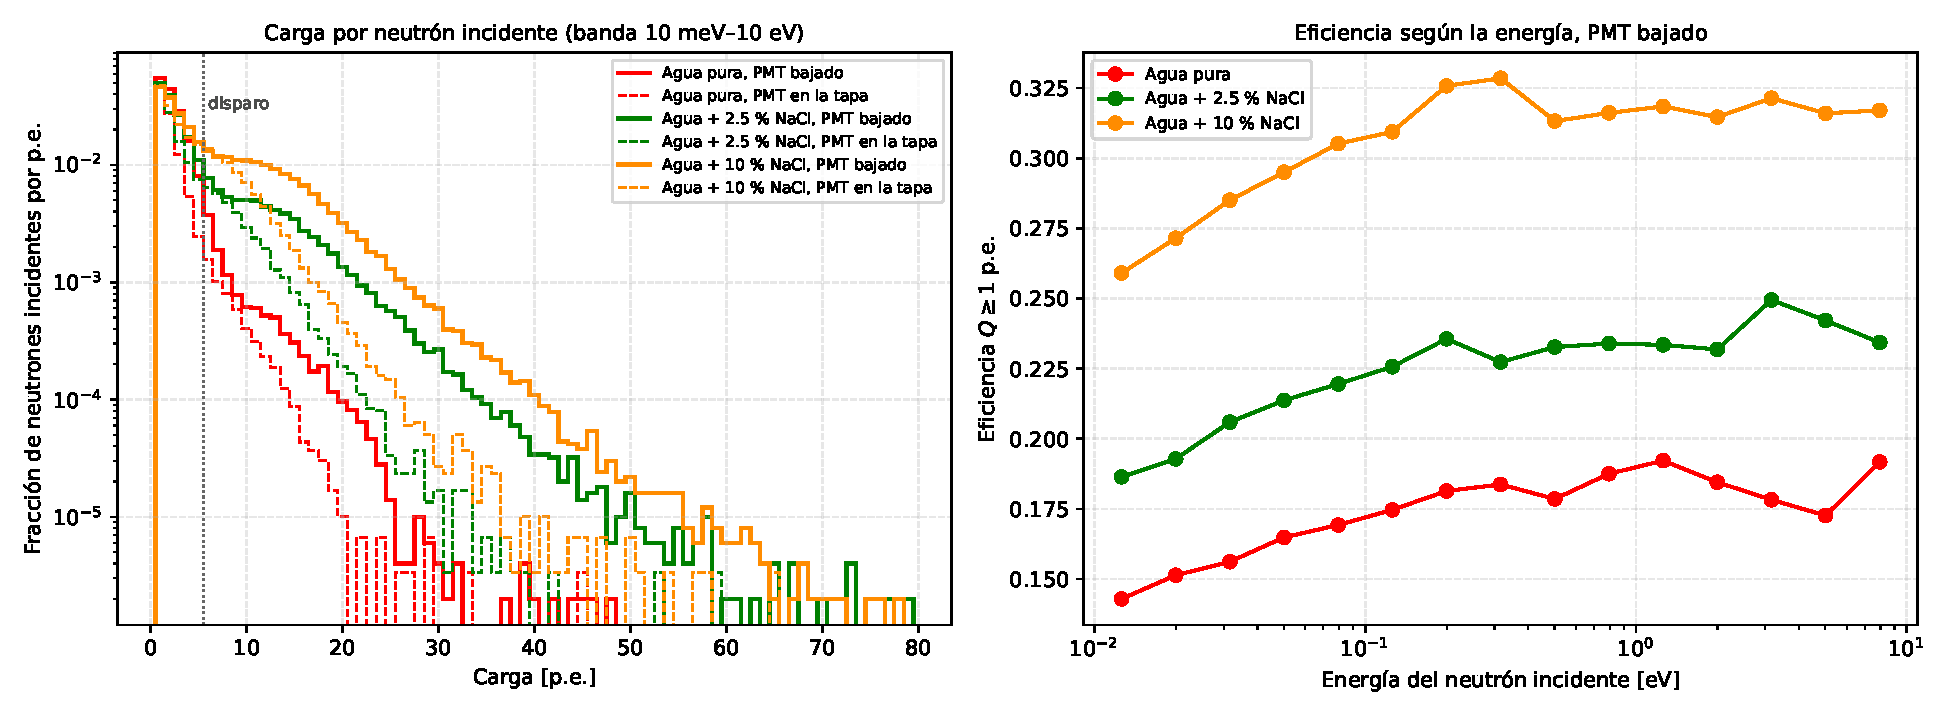
\includegraphics[width=\linewidth]{fig01_carga_eficiencia.pdf}
\caption{Izquierda: carga por neutrón incidente con el PMT bajado (continua) y con el PMT en la tapa (trazos), en la
misma banda; la línea punteada es el disparo aproximado ($\approx$5.5~p.e.\ con $k=650$~ADC/p.e.). Derecha:
eficiencia $Q\geq1$~p.e.\ según la energía del neutrón incidente.}\label{fig:carga}
\end{figure}

\begin{figure}[H]\centering
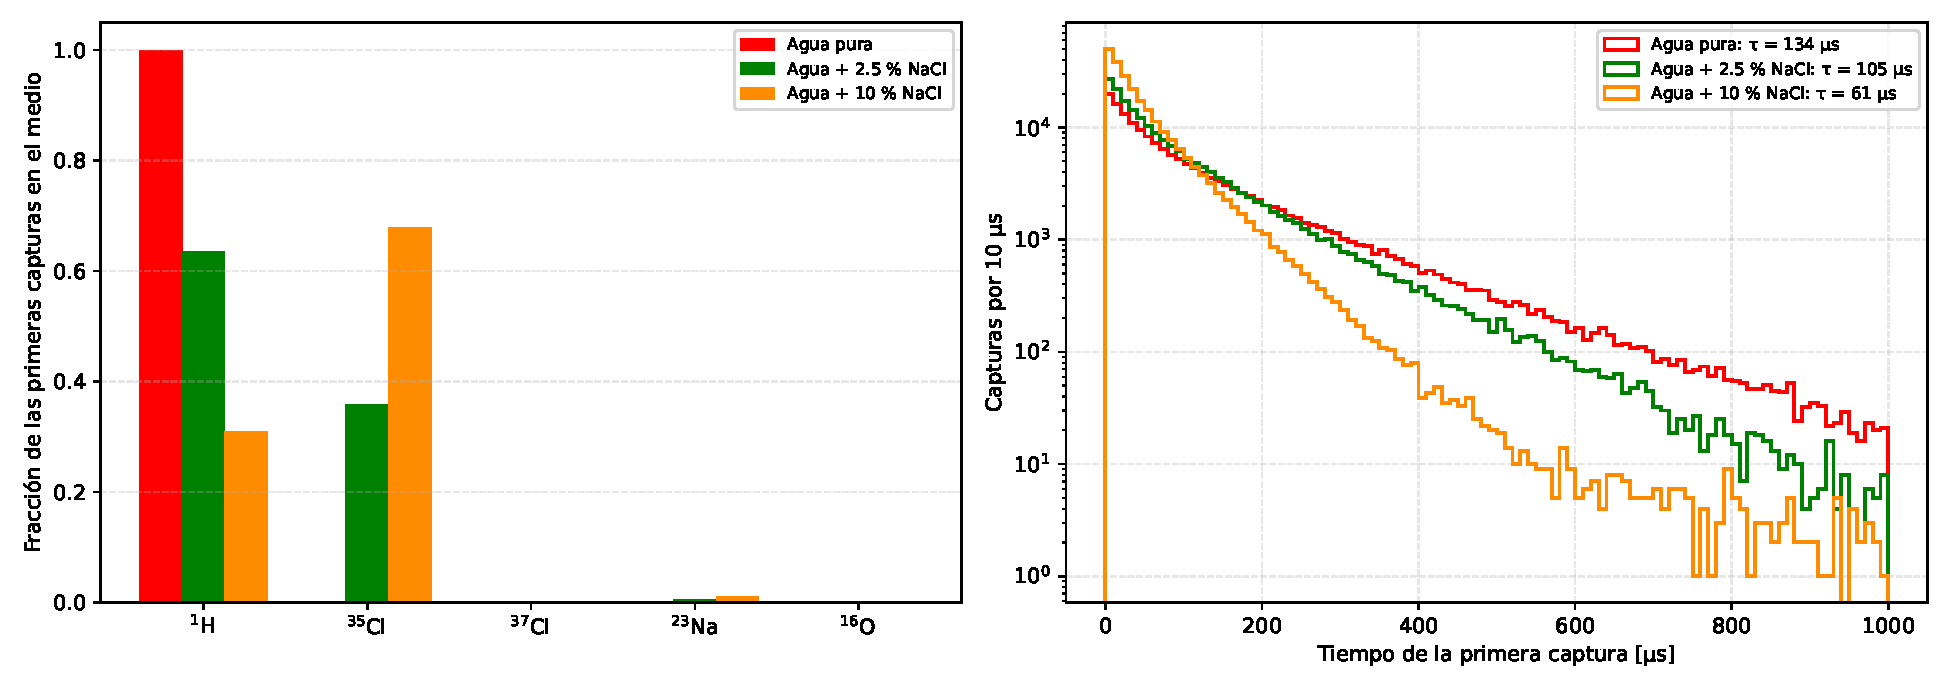
\includegraphics[width=\linewidth]{fig02_capturas.pdf}
\caption{Núcleo de la primera captura y distribución del tiempo de captura.}
\end{figure}

\begin{figure}[H]\centering
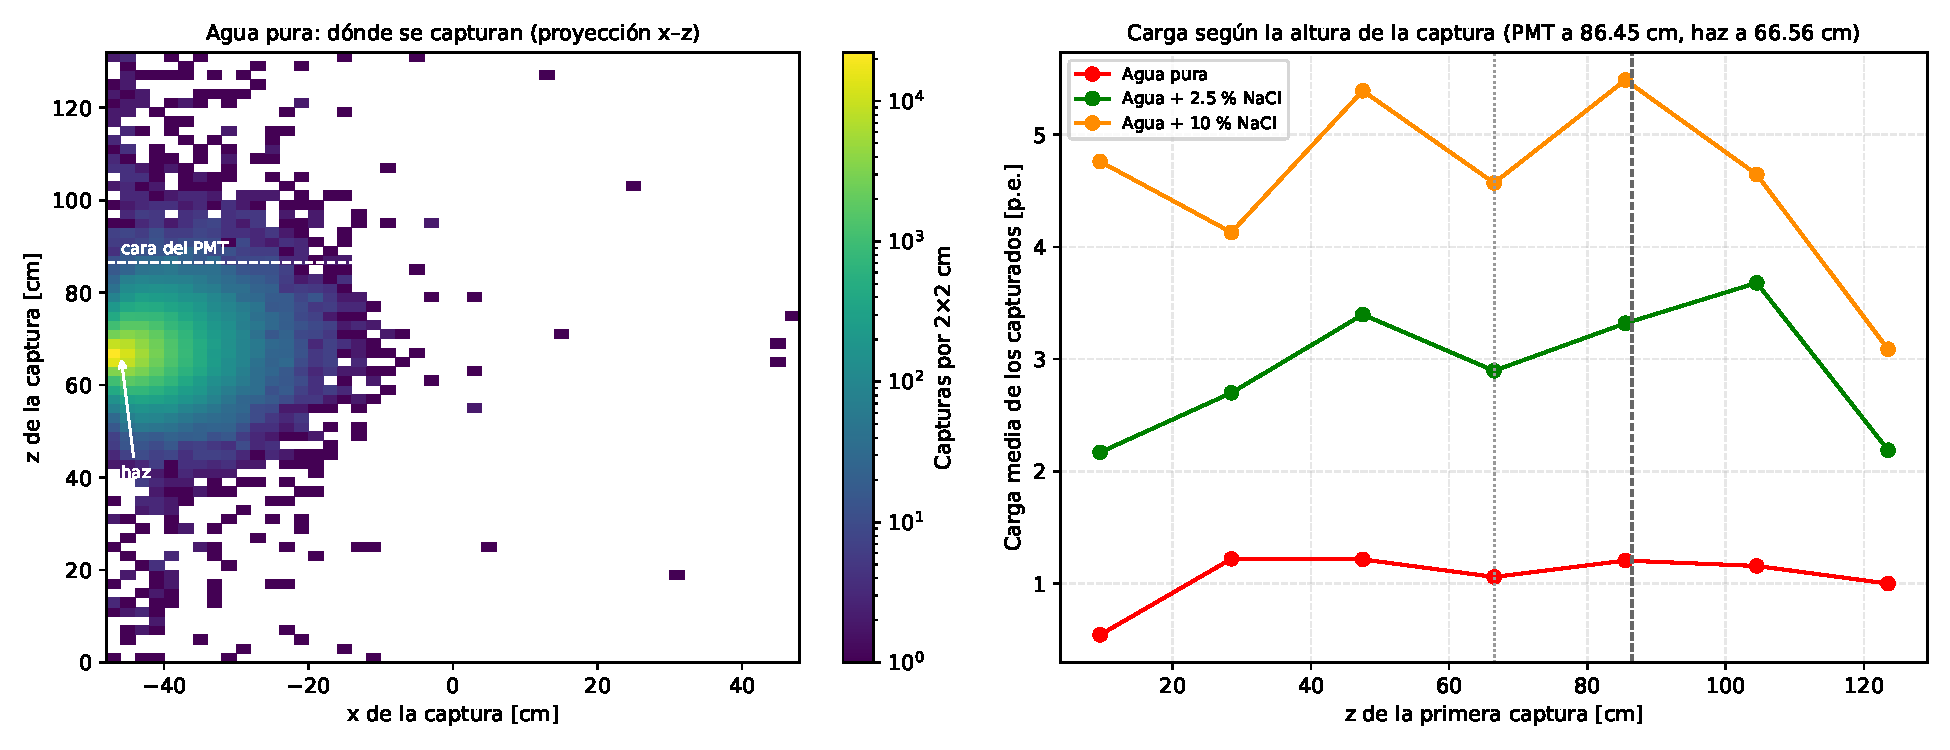
\includegraphics[width=\linewidth]{fig03_posicion_captura.pdf}
\caption{Izquierda: posición de las capturas en agua pura (proyección $x$--$z$, escala logarítmica). Derecha: carga
media de los neutrones capturados según la altura de la captura.}\label{fig:pos}
\end{figure}

\section{Experimento frente a simulación: factores comunes}
\subsection{El método}
Se sigue el método de los cuadernos del prototipo: la carga simulada (p.e.) se lleva a ADC con un solo factor
horizontal $k$ y se escala con un solo factor vertical $N$ (neutrones incidentes en 300~s). Los dos factores son
los mismos para los tres medios. Se ajustan sobre el exceso medido (fuente $-$ fondo, normalizado a 300~s) entre
4500 y 30\,000~ADC, minimizando la dispersión de $\ln(\text{exp}/\text{sim})$; los bins sin simulación cuentan como
0.5 eventos. Se hace de dos maneras:
\begin{enumerate}
\item con solo la resolución de un fotoelectrón (40\,\%), como en los cuadernos;
\item con la electrónica completa (\archivo{respuesta_prototipo.py}): resolución, cociente carga/amplitud medido,
recorte del ADC en 8040 cuentas y disparo con pico $>1200$~ADC.
\end{enumerate}
La carga medida se toma con la ventana del disparo y con el método robusto.

\begin{table}[H]\centering\footnotesize
\tabla{factores_comunes}
\caption{Factores comunes ajustados con el PMT en la tapa (montaje Am-Be completo, $10^6$ n) y con el PMT bajado
(esta corrida). $k/k_\mu$: cociente entre el $k$ ajustado y el que da la calibración con muones del mismo PMT.}\label{tab:fc}
\end{table}

\begin{figure}[H]\centering
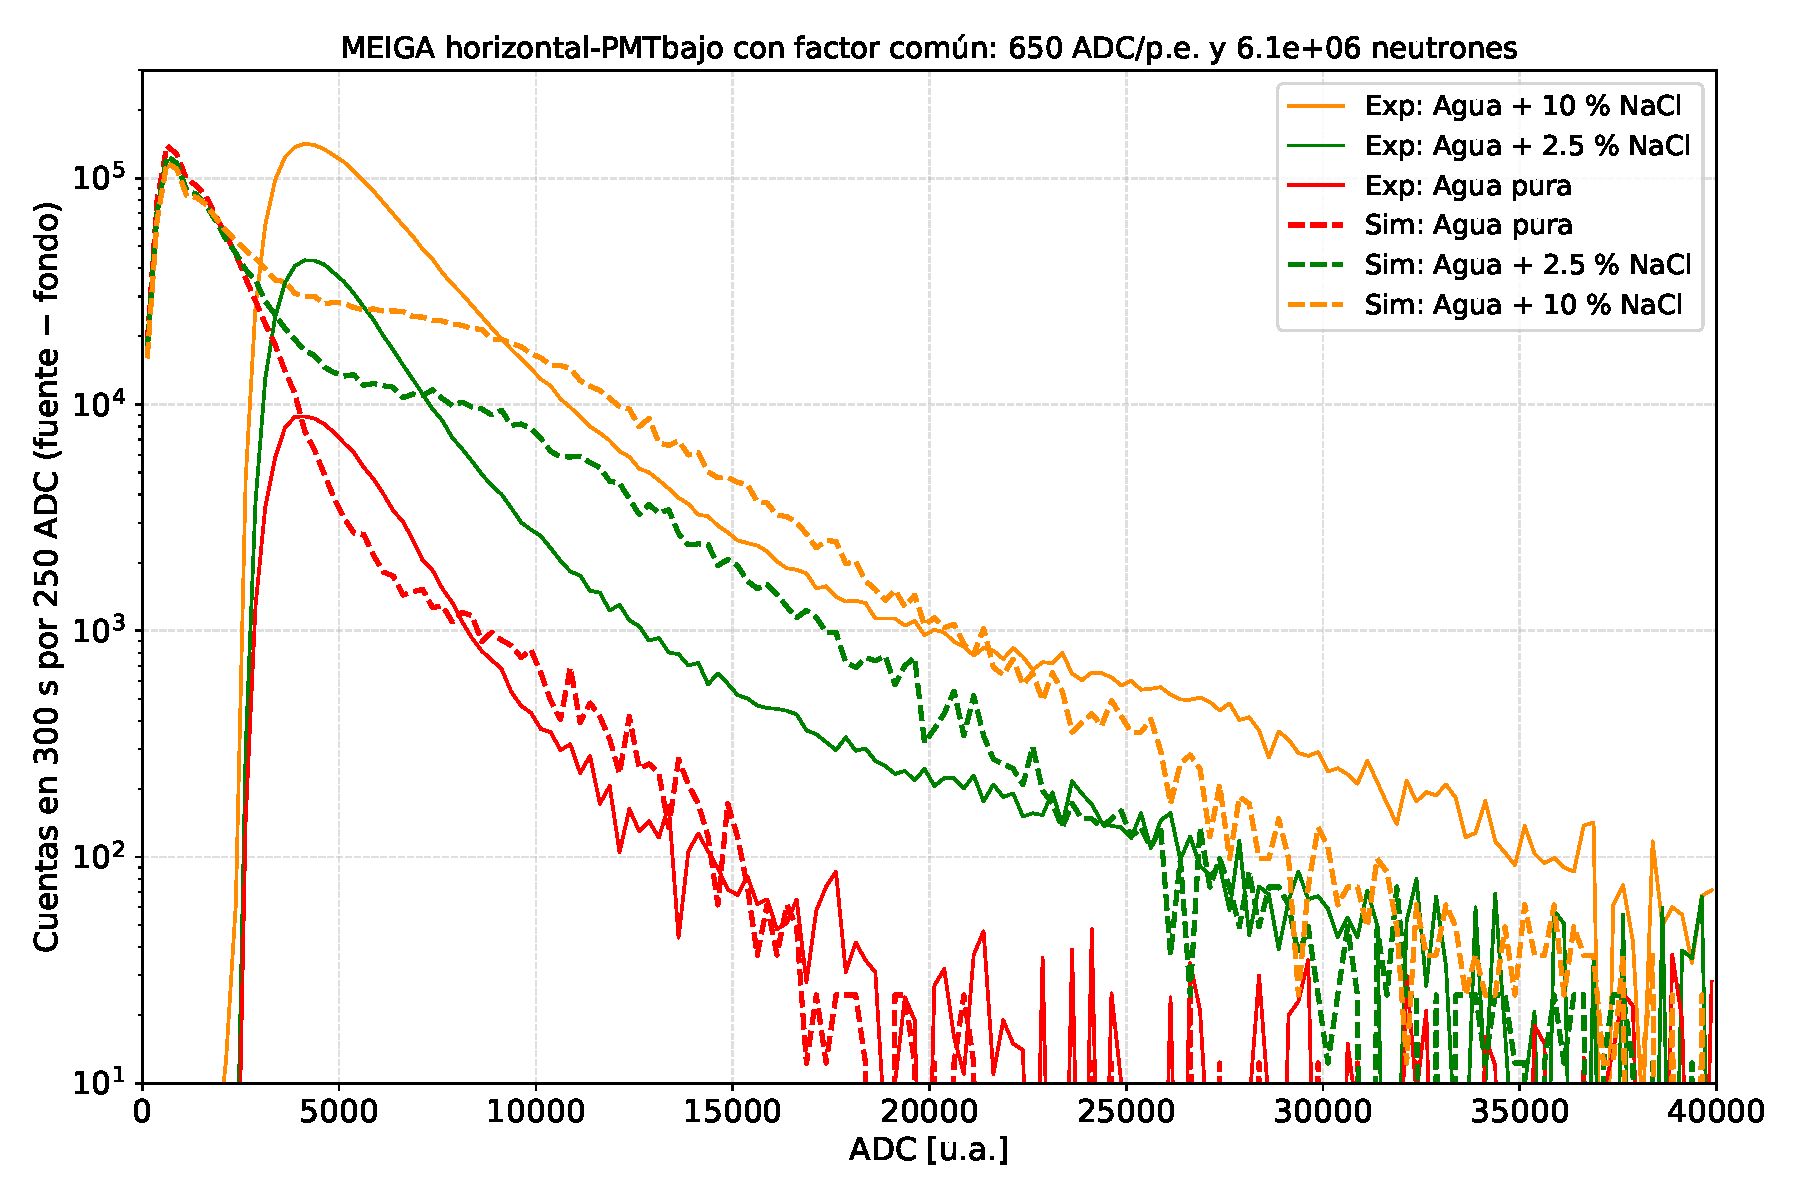
\includegraphics[width=0.85\linewidth]{fig10b_histogramas_factor_comun_horizontal-PMTbajo.pdf}
\caption{Exceso medido (continuas) y simulación con los factores comunes $k=650$~ADC/p.e.\ y $N=6.1\times10^6$
(trazos), con la resolución de 1~p.e.}\label{fig:fc}
\end{figure}

\begin{figure}[H]\centering
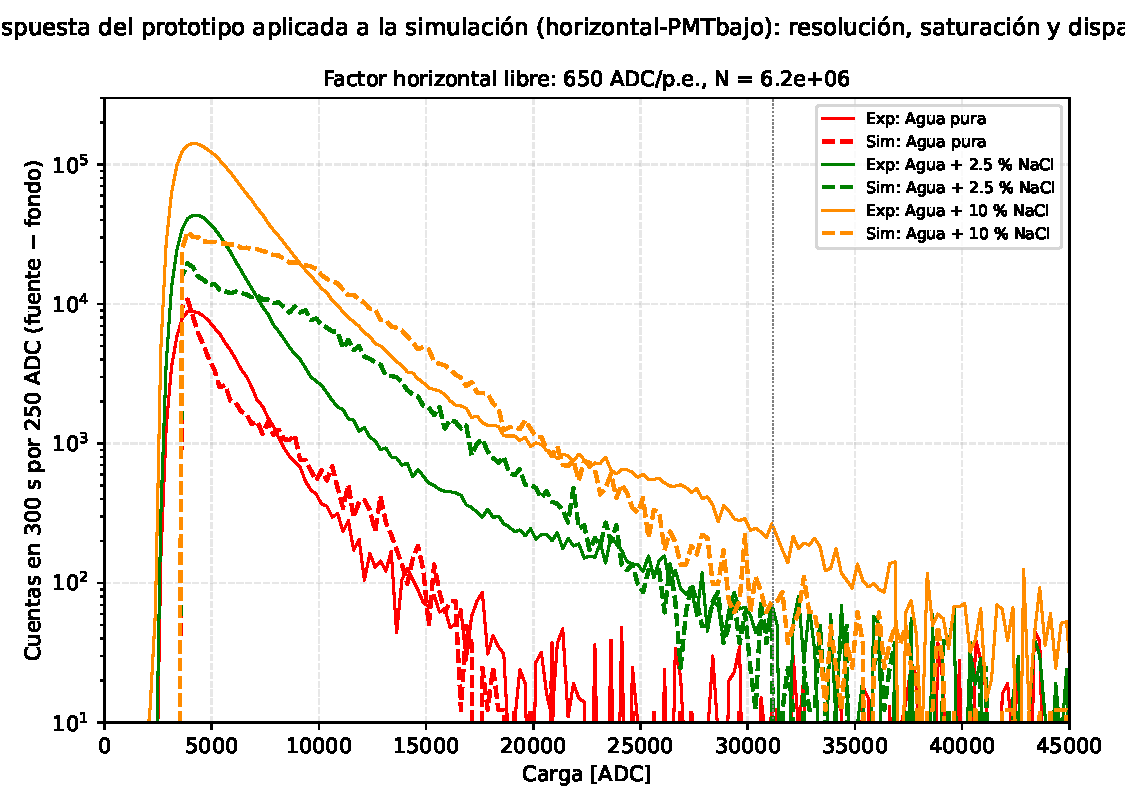
\includegraphics[width=0.6\linewidth]{fig14_respuesta_prototipo_horizontal-PMTbajo.pdf}
\caption{Lo mismo, con la electrónica completa (recorte del ADC y disparo): $k=650$~ADC/p.e.\ y $N=6.2\times10^6$.
La línea punteada vertical es la carga de un pulso recortado en el techo del ADC.}\label{fig:elec}
\end{figure}

\subsection{Resultados}
\begin{itemize}
\item El ajuste da $k=625$--650~ADC/p.e.\ y $N=6.1$--$7.6\times10^6$ neutrones en 300~s. El residuo (0.81--0.83)
es igual al del PMT en la tapa (0.82--0.87): con un par de factores comunes, el PMT bajado describe los datos
igual de bien, no mejor.
\item El $k$ ajustado baja de $\approx$1000 a 650~ADC/p.e.\ al bajar el PMT, aproximadamente en la proporción en que sube la
luz simulada por evento (1.25--1.55 en la carga media). El factor horizontal compensa la luz que falta en la simulación; no es una ganancia física
del PMT.
\item Con la electrónica completa (figura~\ref{fig:elec}) el disparo corta la simulación en $\approx$3.5~kADC,
igual que en los datos, y el agua pura se reproduce en todo el intervalo. En 2.5 y 10\,\% NaCl la simulación es
más ancha que los datos: falta señal en el máximo (4--6~kADC) y sobra entre 8 y 20~kADC. La distancia KS de forma
es 0.18 (pura), 0.35 (2.5\,\%) y 0.30 (10\,\%).
\item Si a cada medio se le deja su propio factor vertical con el $k$ común, $N$ vale 8.4 (pura), 3.9 (2.5\,\%) y
$7.6\times10^6$ (10\,\%). La sal cambia la forma simulada más de lo que cambia la medida, el mismo patrón que con
el PMT en la tapa.
\end{itemize}

\subsection{Prueba de la calibración con muones}
Con 2000 muones verticales de 4~GeV/c en el mismo detector (PMT bajado), el pico de la VEM simulada queda en
581~p.e.\ (305~p.e.\ con el PMT en la tapa). Llevado al pico de muones de las tomas de fondo, da
$k_\mu=68$--70~ADC/p.e., es decir 14.3--14.7~p.e.\ por cada 1000~ADC, con la corrección por recorte.
Antes de mirar el resultado se fijó que esta calibración entraría al informe solo si mejoraba el acuerdo con los
datos. Las condiciones eran tres, y debían cumplirse con los dos métodos de carga:
$0.67\leq k/k_\mu\leq1.5$; $\text{rms}(k_\mu)\leq1.25\,\text{rms}(k)$; y, con $k_\mu$, al menos el 80\,\% de los
bins del intervalo con simulación en los tres medios.

\aviso{\textbf{No pasa}: $k/k_\mu=9.4$--9.8, el rms con $k_\mu$ es 2.5 veces el del ajuste libre, y con $k_\mu$ la
simulación del agua pura no tiene ningún bin entre 4500 y 30\,000~ADC (2.5\,\%: 4\,\%; 10\,\%: 7\,\%). Por eso
este informe usa solo los factores comunes ajustados (\archivo{resultados/decision_calibracion_muones.json}).}

Bajar el PMT no acerca la calibración por muones a los datos: con el PMT en la tapa $k/k_\mu$ era 7.7--8.3, y
ahora es 9.4--9.8. La VEM simulada aumenta casi el doble, pero la luz de los neutrones aumenta mucho menos.

\section{Interpretación}
\begin{itemize}
\item Con factores comunes, la simulación reproduce la forma del agua pura y el orden de los tres medios, con el
mismo residuo en las dos posiciones del PMT. Bajar el PMT da más señal por neutrón, pero no cambia la conclusión
del informe del montaje: la luz medida por evento es $\approx$10 veces la que predice la simulación si se calibra
con muones.
\item La diferencia de forma en los medios con sal (la simulación es más ancha) apunta a que la simulación
sobreestima la contribución de las cascadas del $^{36}$Cl a la carga, o a que en los datos hay un componente que
no depende de la sal, como el de los pulsos estrechos ($\leq16$~ns) observado en el exceso.
\item $N\approx6\times10^6$ neutrones en 300~s se refiere solo a la banda moderada (10~meV--10~eV): no es el número
de neutrones de la fuente. Es $\approx$16 veces el modelo del blindaje para 1~Ci, el mismo orden que con el montaje.
\end{itemize}

\aviso{Dos advertencias. (1) Estas corridas solo contienen la banda moderada del espectro de la fuente: la parte
rápida y la epitérmica alta no están. (2) En MEIGA el PMT cuenta los fotones que entran por cualquier cara del
semielipsoide, también por la cara plana superior; con el PMT sumergido esto puede sobreestimar la luz de los
eventos que ocurren encima del PMT.}

\section{Conclusiones}
\begin{enumerate}
\item Con el PMT bajado y el haz horizontal, la eficiencia por neutrón moderado es 16--29\,\% y la fracción sobre
el disparo, 1.3--14.6\,\%, creciente con la sal. Las capturas en $^{35}$Cl llegan al 68\,\% con 10\,\% NaCl.
\item El método de factores comunes (un $k$ y un $N$ para los tres medios) da $k=650$~ADC/p.e.\ y
$N=6.2\times10^6$, y reproduce el agua pura. Los medios con sal quedan dentro de un factor $\approx2$, con la
simulación más ancha que los datos.
\item La calibración con muones del PMT bajado ($\approx$69~ADC/p.e.) no mejora el acuerdo y no se usa: el factor
horizontal que piden los datos es casi 10 veces mayor.
\end{enumerate}

\paragraph{Reproducción.} Desde \archivo{Analisis-PMT-bajo-horizontal/}; \texttt{M} es
\archivo{../Analisis-montaje-MEIGA/scripts} y \texttt{C} la carpeta de una corrida en el ADATA:
{\footnotesize
\begin{verbatim}
# por medio: pura_horiz, nacl25_horiz, nacl10_horiz
python3 $M/procesar_montaje.py $C pura_horiz resultados
python3 $M/ajuste_factor_comun.py --eventos pura_horiz nacl25_horiz nacl10_horiz \
    --calibracion calibracion_vem_pmtbajo.json --etiqueta horizontal-PMTbajo --salida .
python3 $M/respuesta_prototipo.py --muones <muones PMT bajado> \
    --medio pura resultados/eventos_pura_horiz.npz --medio 2.5 ... --medio 10 ... \
    --etiqueta horizontal-PMTbajo --k-libre --sin-panel-muones --salida .
python3 scripts/decidir_calibracion_muones.py
python3 scripts/analizar_horizontal_pmtbajo.py
\end{verbatim}}
El cuaderno \archivo{Analisis-PMT-bajo-horizontal.ipynb} encadena estos pasos.

\end{document}
